\chapter{Virtualization and Cloud: Part
1}\label{virtualization-and-cloud-part-1}

\section{Virtual Servers}\label{virtual-servers}

\begin{itemize}
\tightlist
\item
  Although Cisco is more known for their networking DEVICES (ROUTERS,
  SWITCHES, FIREWALLS), they also offer HARDWARE SERVERS such as UCS
  (Unified Computing System)
\item
  The largest vendors of HARDWARE SERVERS include Dell, EMC, HPE, and
  IBM
\end{itemize}

\section{Servers Before
Virtualization}\label{servers-before-virtualization}

\begin{figure}
\centering
\pandocbounded{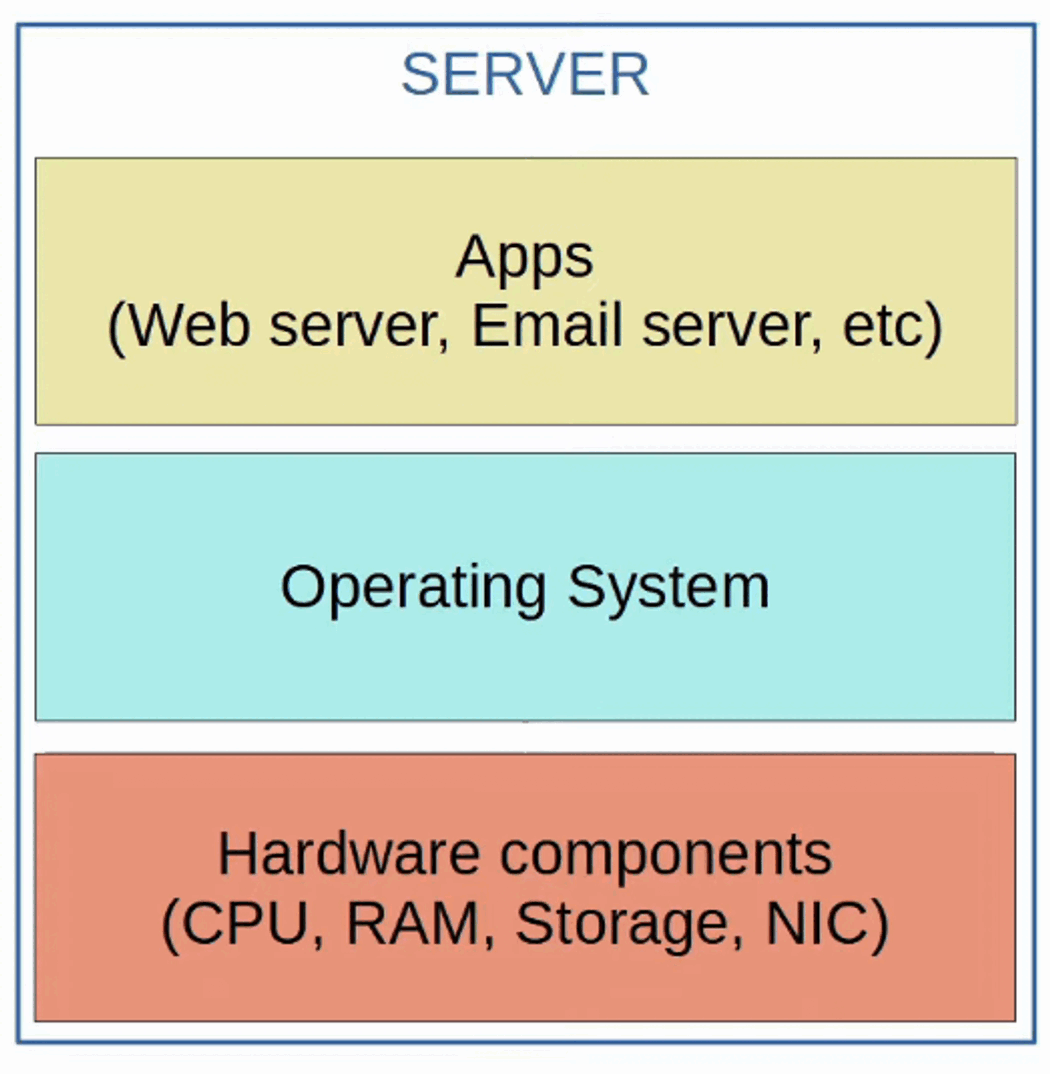
\includegraphics[keepaspectratio,alt={image}]{images/55-virtualizations-and-cloud-part1/img-001.png}}
\end{figure}

\begin{itemize}
\tightlist
\item
  Before VIRTUALIZATION, there was a one-to-one relationship between a
  PHYSICAL SERVER and OPERATION SYSTEM
\item
  In that OPERATING SYSTEM, apps providing SERVICES (such as a WEB
  SERVER, EMAIL SERVER, etc) would run
\item
  One PHYSICAL SERVER would be used for the WEB SERVER, one for the
  EMAIL SERVER, one for the DATABASE SERVER, etc.
\item
  This is inefficient for multiple reasons:

  \begin{itemize}
  \tightlist
  \item
    Each PHYSICAL SERVER is expensive and takes up space, power, etc.
  \item
    The RESOURCES on each PHYSICAL SERVER (CPU, RAM, STORAGE, NIC) are
    typically under-utilized
  \end{itemize}
\end{itemize}

\section{Virtualization (Type 1
Hypervisor)}\label{virtualization-type-1-hypervisor}

\begin{figure}
\centering
\pandocbounded{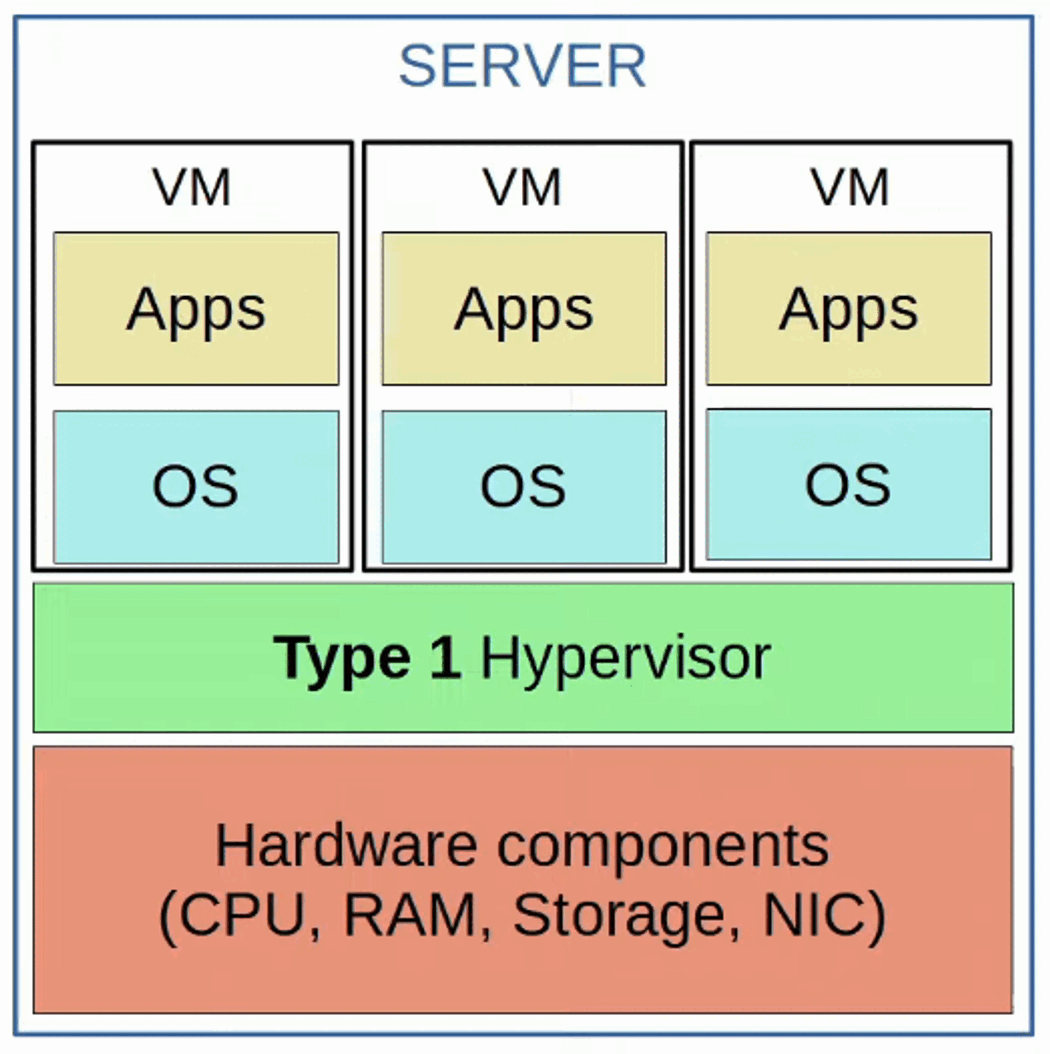
\includegraphics[keepaspectratio,alt={image}]{images/55-virtualizations-and-cloud-part1/img-002.png}}
\end{figure}

\begin{itemize}
\tightlist
\item
  VIRTUALIZATION allows us to break the one-to-one relationships of
  HARDWARE to OS, allowing multiple OS's to run on a single PHYSICAL
  SERVER
\item
  Each INSTANCE is called a VM (Virtual Machine)
\item
  A HYPERVISOR is used to manage and allocate the HARDWARE RESOURCES
  (CPU, RAM, etc.) to each VM
\item
  Another name for a HYPERVISOR is VMM (Virtual Machine Monitor)
\item
  The type of HYPERVISOR which runs directly on top of hardware is
  called a TYPE 1 HYPERVISOR

  \begin{itemize}
  \tightlist
  \item
    Examples include : VMware ESXi, Microsoft Hyper-V, etc.
  \end{itemize}
\item
  TYPE 1 HYPERVISORS are also called \emph{bare-metal hypervisors}
  because they run directly on the hardware (metal).

  \begin{itemize}
  \tightlist
  \item
    Another term is \emph{native hypervisor}
  \end{itemize}
\item
  This is the type of HYPERVISOR used in data center environments
\end{itemize}

\section{Virtualization (Type 2
Hypervisor)}\label{virtualization-type-2-hypervisor}

\begin{figure}
\centering
\pandocbounded{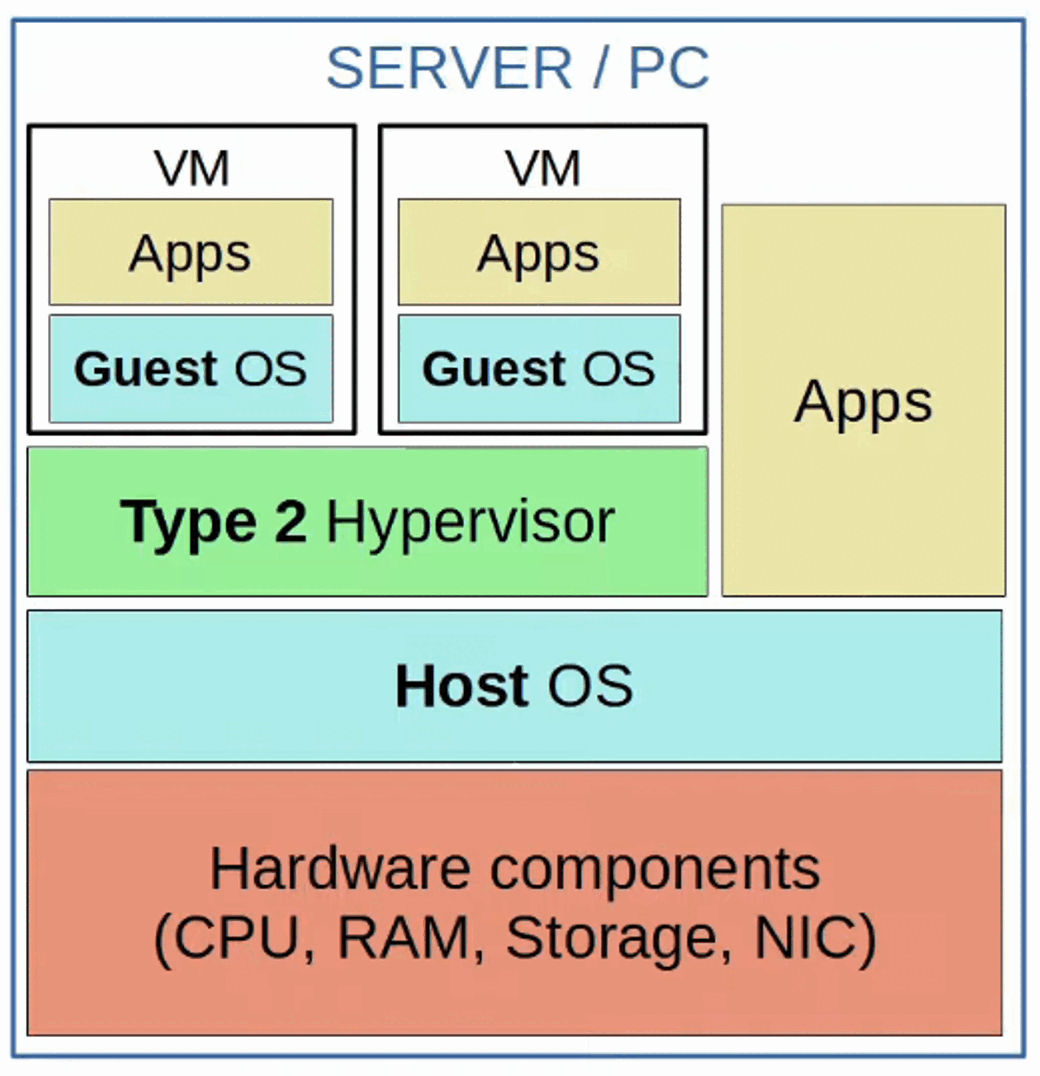
\includegraphics[keepaspectratio,alt={image}]{images/55-virtualizations-and-cloud-part1/img-003.png}}
\end{figure}

\begin{itemize}
\tightlist
\item
  TYPE 2 HYPERVISORS run as a program on an OS like a regular computer
  program

  \begin{itemize}
  \tightlist
  \item
    Examples: VMware Workstation, Oracle Virtualbox, etc
  \end{itemize}
\item
  The OS running directly on the hardware is called the HOST OS
\item
  The OS running in a VM is called a GUEST OS
\item
  Another name for a TYPE 2 HYPERVISOR is \emph{hosted hypervisor}
\item
  Although TYPE 2 HYPERVISORS are rarely used in data center
  environments, they are common on personal-use devices (for example, if
  a MAC/Linux user needs to run an app that is only supported on
  Windows, or vice-versa)
\end{itemize}

WHY VIRTUALIZATION?

\begin{itemize}
\tightlist
\item
  PARTITIONING :

  \begin{itemize}
  \tightlist
  \item
    Run multiple OS's on ONE PHYSICAL MACHINE
  \item
    Divide system resources between VIRTUAL MACHINES
  \end{itemize}
\item
  ISOLATION :

  \begin{itemize}
  \tightlist
  \item
    Provide FAULT and SECURITY ISOLATION at the hardware level
  \item
    Preserve performance with advanced resource controls
  \end{itemize}
\item
  ENCAPSULATION :

  \begin{itemize}
  \tightlist
  \item
    Save the entire state of a virtual machine to files
  \item
    Move and copy virtual machines as easily as moving and copying files
  \end{itemize}
\item
  HARDWARE INDEPENDENCE :

  \begin{itemize}
  \tightlist
  \item
    Provision or migrate any virtual machine to any physical server
  \end{itemize}
\end{itemize}

\begin{figure}
\centering
\pandocbounded{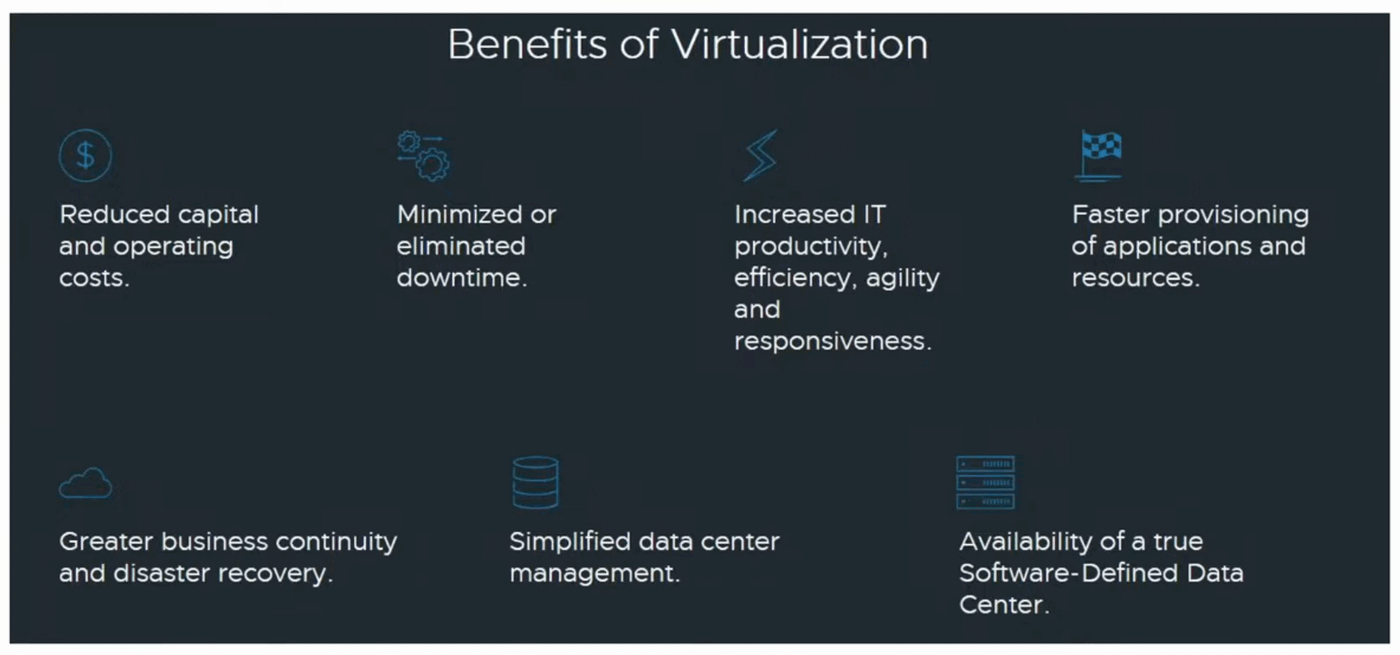
\includegraphics[keepaspectratio,alt={image}]{images/55-virtualizations-and-cloud-part1/img-004.png}}
\end{figure}

\section{Virtual Networks}\label{virtual-networks}

\begin{figure}
\centering
\pandocbounded{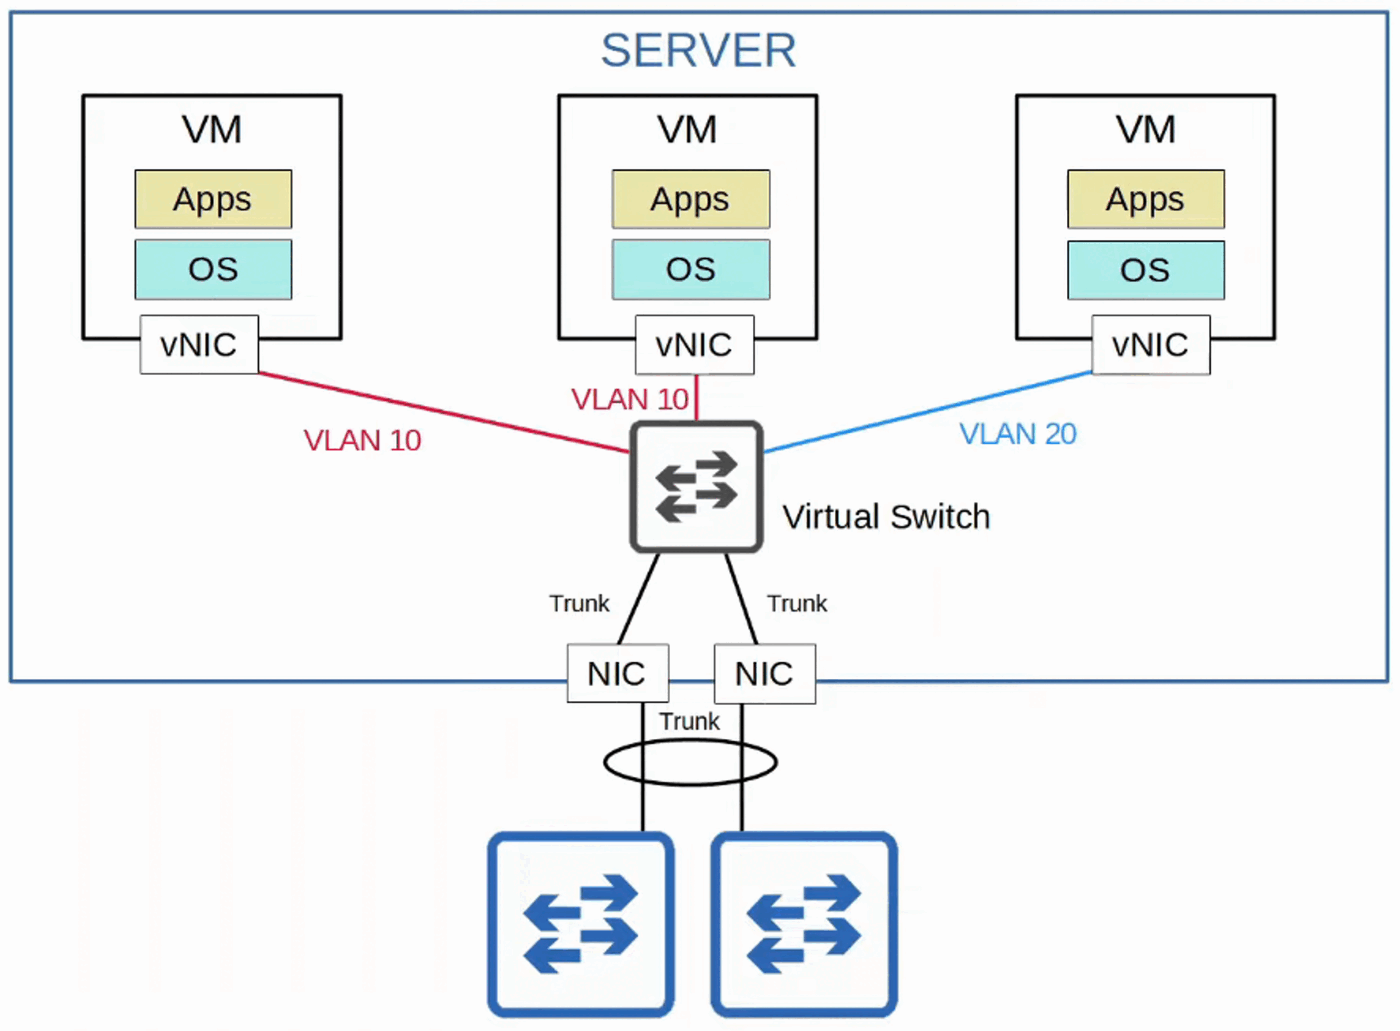
\includegraphics[keepaspectratio,alt={image}]{images/55-virtualizations-and-cloud-part1/img-005.png}}
\end{figure}

\begin{itemize}
\tightlist
\item
  VMs are connected to each other and the EXTERNAL NETWORK via a VIRTUAL
  SWITCH running on the HYPERVISOR
\item
  Just like a regular PHYSICAL SWITCH, the vSWITCH's INTERFACES can
  operate as ACCESS PORTS or TRUNK PORTS and use VLANs to separate the
  VMs at LAYER 2
\item
  INTERFACES on the vSWITCH connect to the PHYSICAL NIC (or NICs) of the
  SERVER to communicate with the EXTERNAL NETWORK
\end{itemize}

\section{Intro to Cloud Computing}\label{intro-to-cloud-computing}

\begin{itemize}
\tightlist
\item
  Traditional IT infrastructure deployments were some combination of the
  following:

  \begin{itemize}
  \tightlist
  \item
    ON-PREMISES

    \begin{itemize}
    \tightlist
    \item
      All SERVERS, NETWORK DEVICES, and other infrastructure are located
      on company property
    \item
      All equipment is purchased and owned by the company using it
    \item
      The company is responsible for the necessary space, power, and
      cooling
    \end{itemize}
  \item
    CO-LOCATION

    \begin{itemize}
    \tightlist
    \item
      Data centers that rent out space for customers to put their
      infrastructure (SERVERS, NETWORK DEVICES)
    \item
      The data center provides the space, electricity, and cooling
    \item
      The SERVERS, NETWORK DEVICES, etc are still the responsibility of
      the end customer, although they are not located on the customer's
      premises
    \end{itemize}
  \end{itemize}
\item
  CLOUD SERVICE provide an alternative that is hugely popular and is
  continuing to grow

  \begin{itemize}
  \tightlist
  \item
    Most people associate ``CLOUD'' with PUBLIC CLOUD PROVIDERS such as
    AWS

    \begin{itemize}
    \tightlist
    \item
      Although this is the most common USE of CLOUD SERVICES, it's not
      the only one
    \end{itemize}
  \end{itemize}
\end{itemize}

\section{Cloud Services}\label{cloud-services}

\begin{itemize}
\tightlist
\item
  The American NIST (National Institute of Standards and Technology)
  defined cloud computing in SP (Special Publication) 800-145
\end{itemize}

\begin{figure}
\centering
\pandocbounded{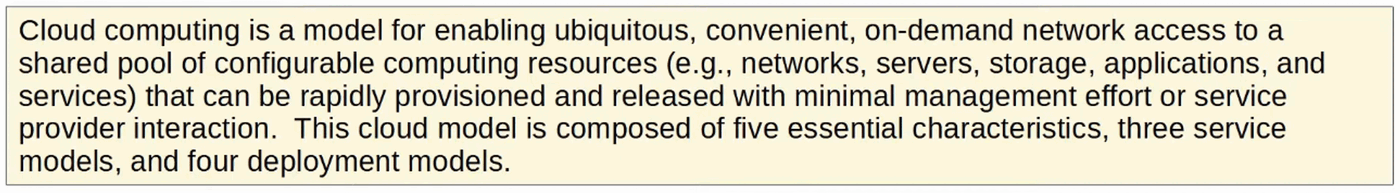
\includegraphics[keepaspectratio,alt={image}]{images/55-virtualizations-and-cloud-part1/img-006.png}}
\end{figure}

\begin{itemize}
\tightlist
\item
  To understand what the CLOUD is, let's look at the following outlined
  in SP 800-145:

  \begin{itemize}
  \tightlist
  \item
    FIVE ESSENTIAL CHARACTERISTICS
  \item
    THREE SERVICE MODELS
  \item
    FOUR DEPLOYMENT MODELS
  \end{itemize}
\end{itemize}

\section{The Five Essential Characteristics of
Cloud}\label{the-five-essential-characteristics-of-cloud}

\begin{itemize}
\tightlist
\item
  ON-DEMAND SELF-SERVICE

  \begin{itemize}
  \tightlist
  \item
    The CUSTOMER is able to use the SERVICE (or stop the SERVICE) freely
    (via a web portal) without direct communication to the SERVICE
    PROVIDER
  \end{itemize}
\item
  BROAD NETWORK ACCESS

  \begin{itemize}
  \tightlist
  \item
    The SERVICE is available through standard NETWORK connections (ie:
    the Internet or PRIVATE WAN) and can be access through many kinds of
    DEVICES
  \end{itemize}
\item
  RESOURCE POOLING

  \begin{itemize}
  \tightlist
  \item
    A POOL of RESOURCES is provided by the SERVICE PROVIDER and when a
    CUSTOMER requests a SERVICE (for example creates a new VM), the
    RESOURCES to fulfill that request are allocated from the shared POOL
  \end{itemize}
\item
  RAPID ELASTICITY

  \begin{itemize}
  \tightlist
  \item
    CUSTOMERS can quickly expand the SERVICE they use in the CLOUD (for
    example: add new VMs, expand STORAGE, etc) from a POOL of RESOURCES
    that appear to be infinite. Likewise, they can quickly reduce their
    SERVICES when not needed
  \end{itemize}
\item
  MEASURED SERVICE

  \begin{itemize}
  \tightlist
  \item
    The CLOUD SERVICE PROVIDER measures the CUSTOMER's usage of CLOUD
    RESOURCES and the CUSTOMER can measure their own use as well.
    CUSTOMERS are charged based on usage (for example: X Dollars per
    Gigabyte of STORAGE per day)
  \end{itemize}
\end{itemize}

\section{The Three Service Models of the
Cloud}\label{the-three-service-models-of-the-cloud}

\begin{figure}
\centering
\pandocbounded{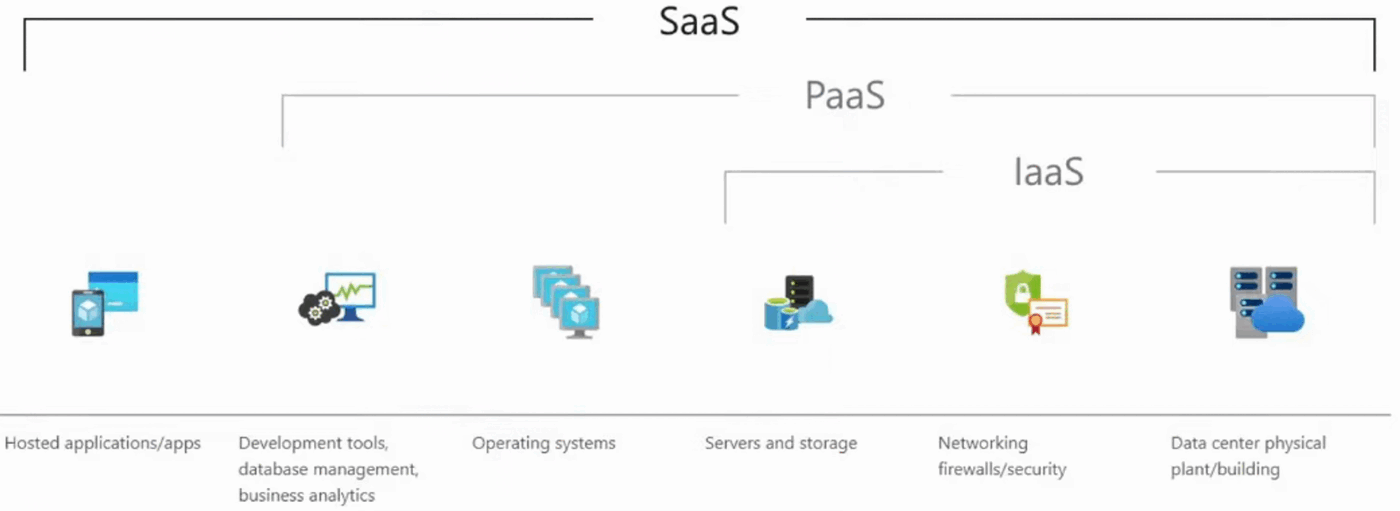
\includegraphics[keepaspectratio,alt={image}]{images/55-virtualizations-and-cloud-part1/img-007.png}}
\end{figure}

\begin{itemize}
\item
  In CLOUD COMPUTING, everything is provided on a ``SERVICE'' model
\item
  For example: rather than the END USER buying a PHYSICAL SERVER,
  mounting it on a rack, installing the hypervisor, creating the VM,
  etc. the SERVICE PROVIDER offers all of this as a SERVICE
\item
  There are a variety of SERVICES referred to as
  ``\_\_\_\_\_\_\_\_\_\_\_ as a SERVICE'' or ``\_\_aaS''
\item
  The THREE SERVICE MODELS of CLOUD COMPUTING are:

  SOFTWARE as a SERVICE (SaaS) - Example : MS Office 365
\end{itemize}

\begin{figure}
\centering
\pandocbounded{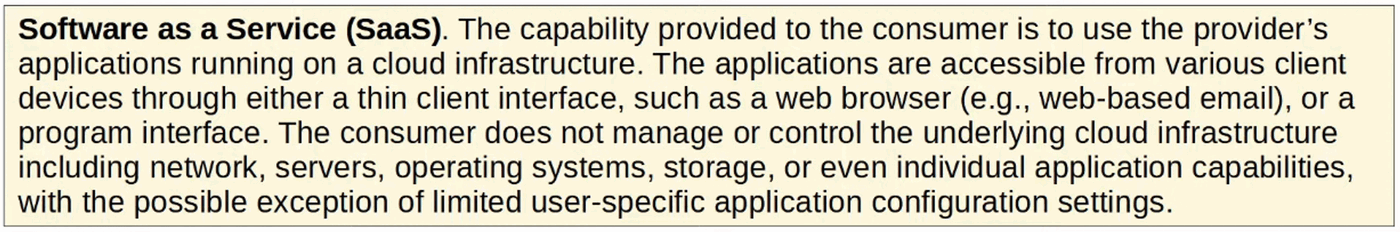
\includegraphics[keepaspectratio,alt={image}]{images/55-virtualizations-and-cloud-part1/img-008.png}}
\end{figure}

\begin{lstlisting}
PLATFORM as a SERVICE (PaaS) - Examples : AWS Lambda and Google App Engine
\end{lstlisting}

\begin{figure}
\centering
\pandocbounded{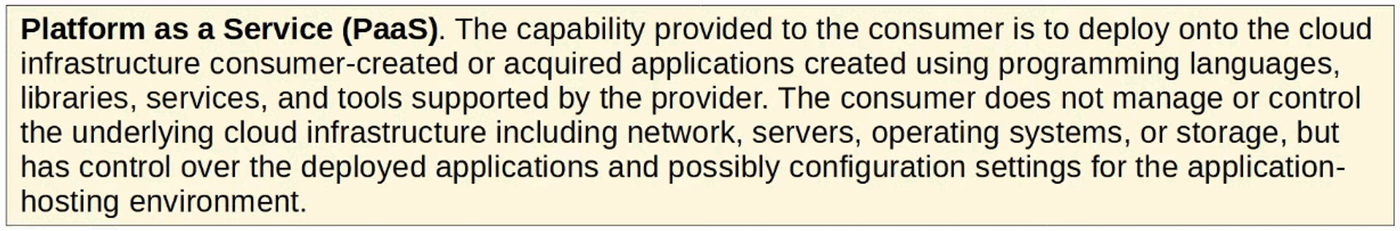
\includegraphics[keepaspectratio,alt={image}]{images/55-virtualizations-and-cloud-part1/img-009.png}}
\end{figure}

\begin{lstlisting}
INFRASTRUCTURE as a SERVICE (Iaas) - Examples: Amazon EC2 and Google Compute Engine
\end{lstlisting}

\begin{figure}
\centering
\pandocbounded{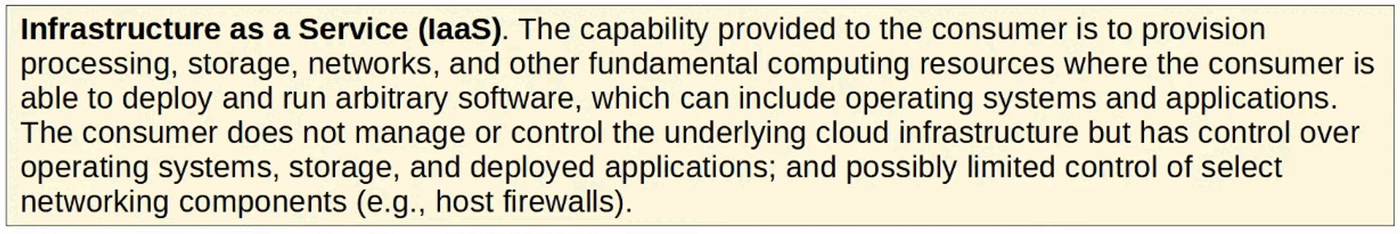
\includegraphics[keepaspectratio,alt={image}]{images/55-virtualizations-and-cloud-part1/img-010.png}}
\end{figure}

\section{Deployment Models}\label{deployment-models}

\begin{itemize}
\item
  Most people assume that ``CLOUD'' means PUBLIC CLOUD PROVIDERS like
  AWS, AZURE, and GCP
\item
  Although ``PUBLIC CLOUD'' is the most common deployment model, it's
  not the ONLY one
\item
  The FOUR DEPLOYMENT MODELS of CLOUD COMPUTING are:
\item
  PRIVATE CLOUD
\end{itemize}

\begin{figure}
\centering
\pandocbounded{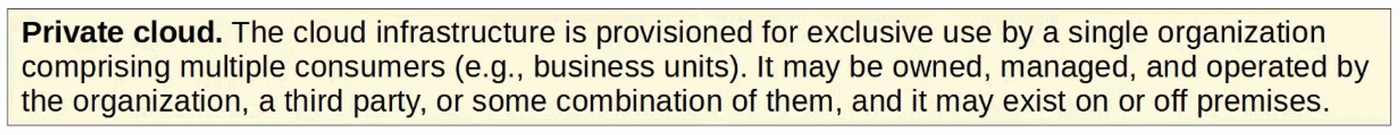
\includegraphics[keepaspectratio,alt={image}]{images/55-virtualizations-and-cloud-part1/img-011.png}}
\end{figure}

\begin{itemize}
\item
  PRIVATE CLOUDS are generally only used by large enterprises
\item
  Although the CLOUD is PRIVATE, it may be owned by a THIRD PARTY

  \begin{itemize}
  \tightlist
  \item
    For example: AWS provides PRIVATE CLOUD SERVICES for the American
    DoD
  \end{itemize}
\item
  PRIVATE CLOUDS may be ON or OFF PREMISES

  \begin{itemize}
  \tightlist
  \item
    Many people assume ``CLOUD'' and ``ON-PREM'' are two different
    things but that is not always the case
  \end{itemize}
\item
  The same kind of SERVICES offered are the same as in PUBLIC CLOUDS
  (SaaS, PaaS, IaaS) but the infrastructure is reserved for a SINGLE
  ORGANIZATION
\item
  COMMUNITY CLOUD
\end{itemize}

\begin{figure}
\centering
\pandocbounded{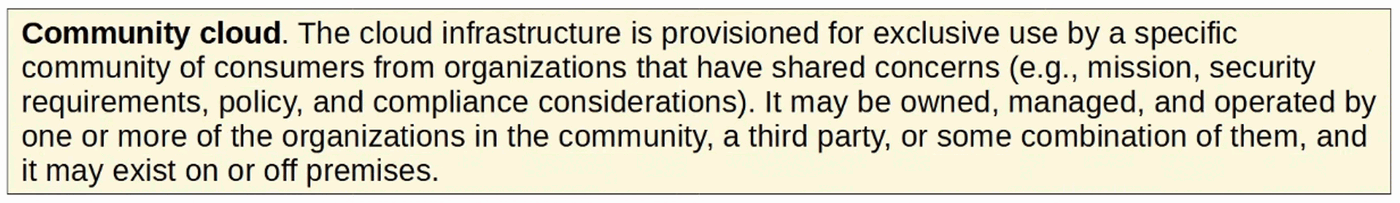
\includegraphics[keepaspectratio,alt={image}]{images/55-virtualizations-and-cloud-part1/img-012.png}}
\end{figure}

\begin{itemize}
\item
  Least common CLOUD deployment
\item
  Similar to PRIVATE CLOUD, but the INFRASTRUCTURE is reserved for use
  by a SPECIFIC GROUP or ORGANIZATION
\item
  PUBLIC CLOUD
\end{itemize}

\begin{figure}
\centering
\pandocbounded{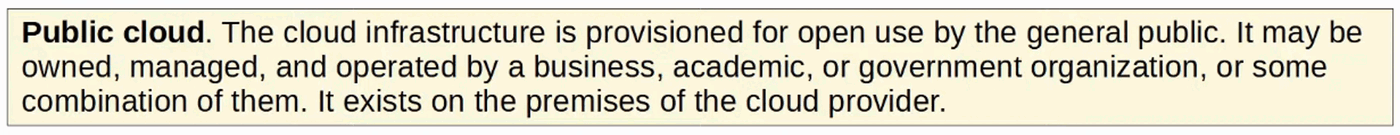
\includegraphics[keepaspectratio,alt={image}]{images/55-virtualizations-and-cloud-part1/img-013.png}}
\end{figure}

\begin{itemize}
\tightlist
\item
  The most common CLOUD deployment
\item
  Popular PUBLIC CLOUD service providers include:

  \begin{itemize}
  \tightlist
  \item
    AWS
  \item
    MS AZURE
  \item
    GCP (Google Cloud Platform)
  \item
    OCI (Oracle Cloud Infrastructure)
  \item
    IBM Cloud
  \item
    Alibaba Cloud
  \end{itemize}
\item
  HYBRID CLOUD
\end{itemize}

\begin{figure}
\centering
\pandocbounded{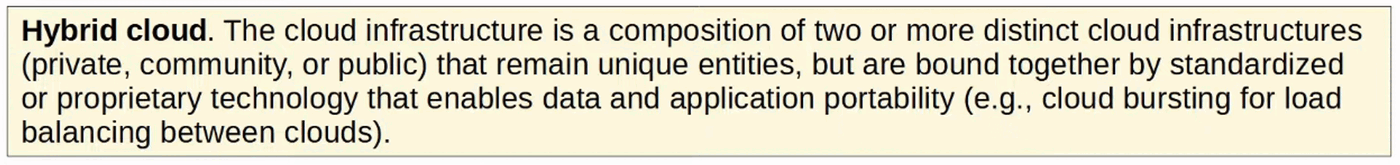
\includegraphics[keepaspectratio,alt={image}]{images/55-virtualizations-and-cloud-part1/img-014.png}}
\end{figure}

\begin{lstlisting}
- Basically ANY combination of the preview THREE DEPLOYMENT TYPES
- Example: A PRIVATE CLOUD which can offload to a PUBLIC CLOUD when necessary
\end{lstlisting}

\section{Benefits of Cloud Computing}\label{benefits-of-cloud-computing}

\begin{itemize}
\tightlist
\item
  COST

  \begin{itemize}
  \tightlist
  \item
    CapEx (Capital Expense) of buying HARDWARE and SOFTWARE, setting up
    DATA CENTERS, etc. are reduced or eliminated
  \end{itemize}
\item
  GLOBAL SCALE

  \begin{itemize}
  \tightlist
  \item
    CLOUD SERVICES can scale GLOBALLY at a rapid pace. SERVICES can be
    set up and offered to CUSTOMERS from a geographic location close to
    them
  \end{itemize}
\item
  SPEED / AGILITY

  \begin{itemize}
  \tightlist
  \item
    SERVICES are provide ON DEMAND and vast amounts of RESOURCES can be
    provisioned within minutes
  \end{itemize}
\item
  PRODUCTIVITY

  \begin{itemize}
  \tightlist
  \item
    CLOUD SERVICES remove the need for many time-consuming tasks such as
    procuring physical servers, racking them, cabling, installing and
    updating equipment, etc.
  \end{itemize}
\item
  RELIABILITY

  \begin{itemize}
  \tightlist
  \item
    Backups in the CLOUD are very easy to perform. Data can be mirrored
    at multiple sites in different geographic locations to support
    disaster recovery
  \end{itemize}
\end{itemize}

\section{Connection to Public Clouds}\label{connection-to-public-clouds}

\begin{figure}
\centering
\pandocbounded{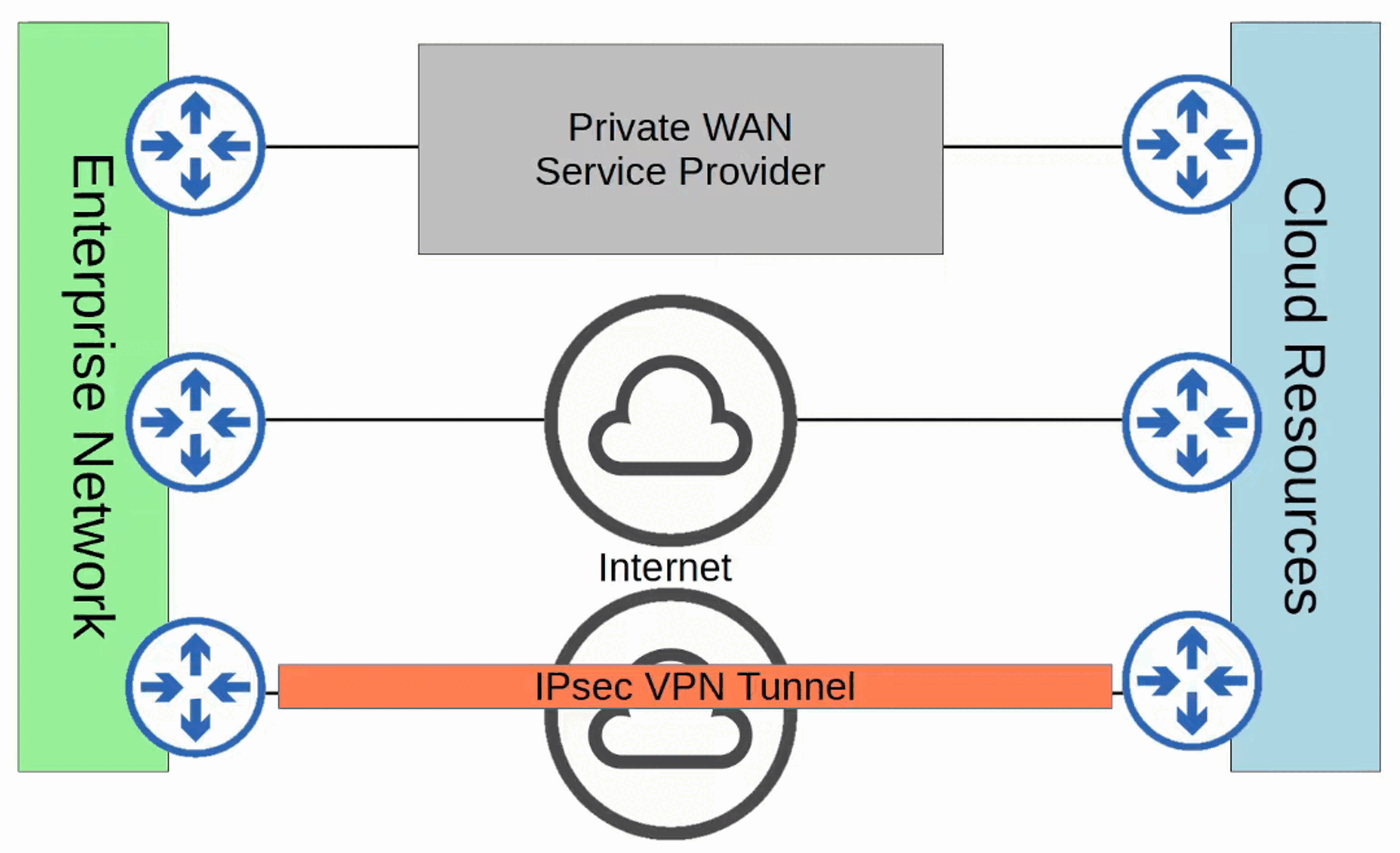
\includegraphics[keepaspectratio,alt={image}]{images/55-virtualizations-and-cloud-part1/img-015.png}}
\end{figure}
